\documentclass[a4paper]{article}

\usepackage[portuguese]{babel} \usepackage[utf8]{inputenc}
%\usepackage{indentfirst}
\usepackage{graphicx}
\usepackage{verbatim}
\usepackage[T1]{fontenc}
\usepackage{wrapfig}
\usepackage[tmargin=1.2in,bmargin=1in]{geometry}
\usepackage{listingsutf8}
\usepackage[utf8]{inputenc}
\usepackage{color}
\usepackage{ucs}
\lstset{literate=%
{æ}{{\ae}}1
{å}{{\aa}}1
{ø}{{\o}}1
{Æ}{{\AE}}1
{Å}{{\AA}}1
{Ø}{{\O}}1
}
\lstset{extendedchars=\true}
\lstset{inputencoding=ansinew}

\begin{document}

\setlength{\textwidth}{16cm} \setlength{\textheight}{22cm}

\title{\Huge\textbf{Protocolo de Ligação de
    Dados}\linebreak\linebreak\linebreak\linebreak \Large\textbf{Relatório \\
    Trabalho1}\linebreak\linebreak\linebreak
\includegraphics[height=6cm,
    width=7cm]{feup.pdf}\linebreak \linebreak \Large{Mestrado Integrado em
    Engenharia Informática e Computação} \linebreak \linebreak \Large\textbf{Redes de
Computadores}\linebreak}

\author{Hugo Ari Rodrigues Drumond --- 201102900 --- hugo.drumond@fe.up.pt \\
    José Pedro Pereira Amorim --- 201206111 --- ei12190@fe.up.pt \\ João
    Ricardo Pintas Soares --- 201200740 ---
    ei12039@fe.up.pt\linebreak\linebreak\linebreak \\ \\ Faculdade de
    Engenharia da Universidade do Porto \\ Rua Roberto Frias, 4200--65 Porto,
    Portugal \linebreak\linebreak\linebreak \linebreak\linebreak\vspace{1cm}}
    \maketitle \thispagestyle{empty}

\newpage

\section{Introdução}
%indicação dos objectivos do trabalho e do relatório; descrição da lógica do
%relatório com indicações sobre o tipo de informação que poderá ser encontrada
%em cada uma secções seguintes
Este trabalho laboratorial, desenvolvido no âmbito da Unidade Curricular de
Redes de Computadores (RCOM), teve como objetivo implementar um protocolo de
ligação de dados, do tipo acknowledged connection-oriented, e testá-lo em
diversas situações de stress de modo a verificar a sua robustez. Ao longo deste
relatório, serão descritos os aspetos fundamentais do referido trabalho,
permitindo obter um conhecimento detalhado deste. Será apresentada a
arquitetura, estrutura do código, casos de uso principais, protocolo de ligação
lógica e de aplicação. No mesmo sentido, serão apresentadas a validação dos
resultados e os elementos de valorização.

\section{Arquitectura}
%blocos funcionais e interfaces
O nosso software foi desenvolvido de maneira a tirar o máximo proveito da
estratégia de encapsulamento. O que permite: modificar, fazer novas
implementações, alterar técnicas de integridade de dados, etc, sem que haja
incompatibilidades ou quebra das interfaces de cada camada. Embora esta ideia
de isolamento tenha surgido nas linguagens de programação orientadas a objetos,
o código em C permite seguir este ideal pelo uso da palavra static. Tal, faz
com que um elemento só seja visível no ficheiro onde está declarado e definido.
A técnica usada pelo nosso código foi declarar a API (funções e estruturas de
retorna de informação public) de cada camada (classe) nos headers. E, nos
respetivos ficheiros de código fazer a definição da API\@; e a declaração e
definição das funções e estruturas auxiliares e de controlo com a palavra
static (private).
\\\newline\textbf{Resultando no seguinte esboço arquitectural:}\\\newline
\centerline{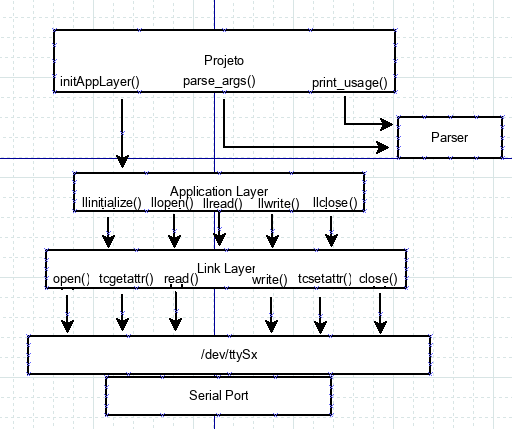
\includegraphics{API.png}}

\section{Estrutura do código}
%APIs, principais estruturas de dados, principais funções e sua relação com a
%arquitetura

\subsection{Organização dos ficheiros e código}
\centerline{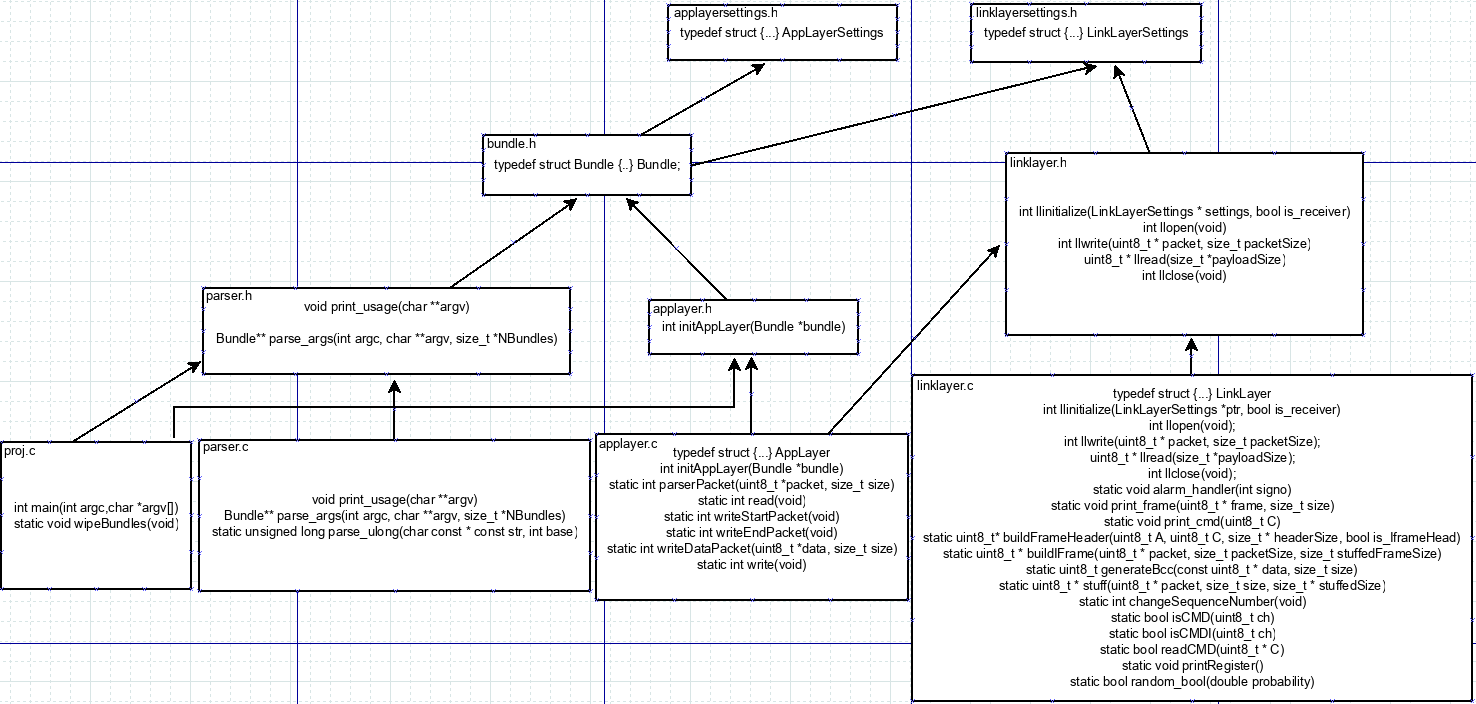
\includegraphics[scale=0.70]{organizacaoFicheirosECodigo.png}}

\subsection{Estruturas}
\begin{figure}[h]
    \centering
    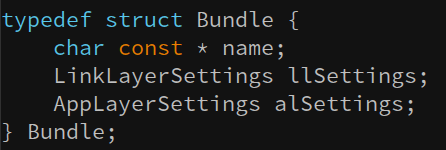
\includegraphics[width=0.45\textwidth]{bundleStruct.png}
    \caption{Estrutura Bundle presente no ficheiro \textit{bundle.h}}
\end{figure}
No \textit{bundle.h} encontra-se uma estrutura chamada Bundle cujo objetivo é
guardar os settings que recebemos da linha de comandos. O name é um nome a que
queremos chamar ao Bundle, e as estruturas constituintes do Bundle são para os
settings de cada camada. O LinkLayerSettings está declarado no ficheiro
\textit{linklayersettings.h} e contém os seguintes argumentos: port, timeout,
numAttempts, payloadSize e baudrate.
\begin{figure}[h]
\centering
    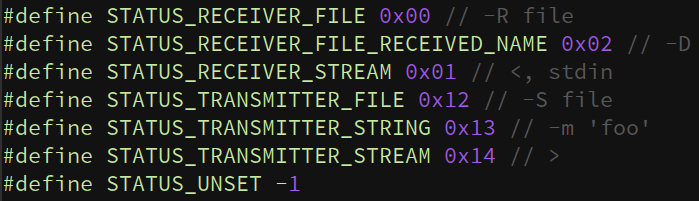
\includegraphics[width=0.45\textwidth]{status.png}
    \caption{Defines modo de operação e tipo IO no ficheiro
    applayersettings.h}
\end{figure}\\
O AppLayerSettings está declarado no ficheiro \textit{applayersettings.h} e
contém os seguintes argumentos: status, packetBodySize, filename e um union Io
que pode ser um apontador para um ficheiro, para uma string ou nulo. Para além
disso, encontram-se lá defines que o parser usa para indicar como aceder ao
Union Io e qual o modo de operação.\\\newline

As estruturas mais importantes do nosso programa são: Applayer e LinkLayer.
Estão presentes, respetivamente, nos ficheiros: \textit{applayer.c} e
\textit{linklayer.c}.\\
\begin{figure}[h]
\centering
    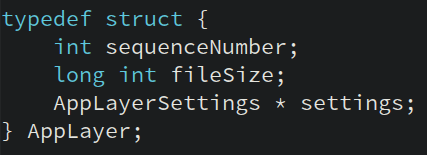
\includegraphics[width=0.45\textwidth]{applayerStruct.png}
    \caption{Estrutura AppLayer presente no ficheiro applayer.c}
\end{figure} \\
Na estrutura Applayer: usamos sequenceNumber para que possamos identificar se
houve algum pacote de dados perdido, e se tal acontecer recuperar desse erro;
fileSize é preenchido com o tamanho do ficheiro a transmitir ou vai sendo
atualizado consoante recebemos informação, para depois compararmos com o pacote
de controlo que vem no fim; e, settings que aponta para um estrutura
AppLayerSettings que foi preenchida pelo parser.\\
\begin{figure}[h]
\centering
    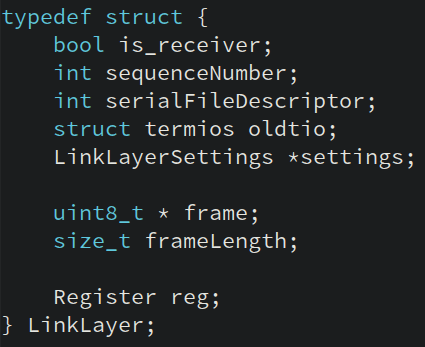
\includegraphics[width=0.45\textwidth]{linklayerStruct.png}
    \caption{Estrutura LinkLayer presente no ficheiro linklayer.c}
\end{figure}
\\ No
caso de LinkLayer: is\_receiver indica o modo de operação; sequenceNumber, a
trama de informação esperada ou a enviar; serialFileDescriptor, o descritor da
porta série aberta; oldtio, informação da porta série a ser reposta no fim da
conexão; settings, apontador para uma estrutura do tipo LinkLayerSettings onde
se encontram as configurações passadas pela linha de comandos que só interessam
a esta camada; frame, apontador para uma trama de informação unstuffed criada
na função \textit{llinitialize} com o tamanho máximo esperado; frameLength,
tamanho da trama de informação recebida; finalmente, temos uma estrutura
chamada Register que guarda ocorrências.

%\begin{wrapfigure}{R}{0.45\textwidth}
%\centering
    %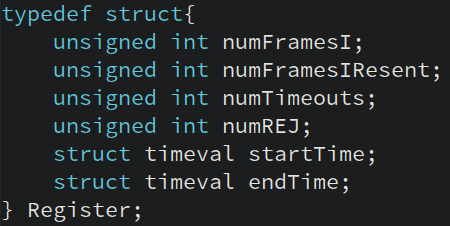
\includegraphics[width=0.45\textwidth]{registerStruct.png}
    %\caption{Estrutura de registo de ocorrências presente no ficheiro
    %linklayer.c}
%\end{wrapfigure}

\subsection{Funções}
\subsubsection{linklayer}
\textbf{\textit{static bool readCMD(uint8\_t * C);}}\\
Esta é a função mais importante do nosso código, e tem o objetivo de reconhecer
qualquer comando válido, seja ele uma trama de dados ou de controlo. É
retornado true se for encontrada uma sequência de bytes válida, isto é, uma
trama bem formada em todos os sentidos; *C, sendo C o endereço de um variável
criada por quem chamou a função. É preenchido com o tipo de comando quando
estamos no estado apropriado, por exemplo: C\_DISC, C\_UA, C\_I\_N, C\_RR, etc.
Progredi-se na máquina de estados quando há um byte bom. Ou retrocede-se quando
há algum byte não esperado. O destuffing, tal como a verificação da integridade
dos dados é feita nesta função. Há uma divergência na máquina de estados que é
consequência de haver dois tipos de tramas. Quando estamos nesse estado e
recebemos um F, e sendo *C um comando da trama de controlo é retornado true,
que simboliza que foi recebido uma sequência válido no tempo configurado para o
alarm. De forma semelhante, é feita a verificação para o caso da trama de
informação. Se estivermos no estado divergente e se *C for um comando válido
para essa trama e o byte recebido for diferente de F dá-se início ao processo
de preenchimento do membro frame da estrutura linkLayer. Sem stuffing mas com
todos os bytes constituintes da trama. É também nesta parte do código onde se
pode gerar erros de teste nas tramas com um dada probabilidade. A estratégia
tomada foi alterar o BBC1(Header) ou o BBC2(Body) no caso da função de
probabilidade \textit{random\_bool(double probabilidade)} tiver retornado true.
As tramas de Informação com o cabeçalho bom mas com BBC errado no campo de
dados são tratadas de forma especial. É também retornado true, no entanto o
llread terá de verificar se o último byte da trama lida (linkLayer.frame) é F
ou não. Porque o F só é adicionado se a trama não tiver erros. Cabe ao
\textit{llopen}, \textit{llread}, \textit{llwrite} e ao \textit{llclose}
decidir o que fazer, consoante o tipo de comandos que recebem, *C, sempre
analisando o retorno.\\

\noindent\textbf{\textit{int llinitialize(LinkLayerSettings *ptr, bool
is\_receiver);}}\\ Esta função, tem de ser corrida antes de qualquer outra, e
tem o objetivo de: preencher os dados iniciais da estrutura linkLayer; instalar
o signal handler; e, alocar memória para linkLayer.frame. De início usámos a
função signal (que está deprecada), mas acabámos por mudar para função
sigaction porque após um sinal alarm o handler levava reset. Resultado num
crash do programa. Todos os argumentos são usados para inicializar valores na
estrutura linkLayer.\\

\noindent\textbf{\textit{int llopen(void);}}\\ Abre a porta série e configura-a
com os settings necessários passados pela linha de comandos, presentes em
linkLayer.settings->{opção}. E guarda as configurações antigas para posterior
restauração. Na parte final do código temos um conjunto de ifs dentro do while
de tentativas em que se trata do processo inicial de estabelecimento da
conexão, que depende do modo de operação. Aproveita a função \textit{readCMD}
para assim evitar criar outra máquina de estados só para este caso específico.
Optámos por tratar do caso especial da trama de controlo UA poder ser perdida
ou haver timeout do emissor no \textit{llread}, uma vez que poderíamos
desperdiçar algum tempo nesta função à espera de alguma trama.\\

\noindent\textbf{\textit{uint8\_t* llread(size\_t *payloadSize);}}\\ Trata de
retornar a payload com um determinado tamanho indicado por *payloadSize à
applayer. A estrutura da função é semelhante à do \textit{llwrite}, no entanto
é bem mais extensa. Um conjunto de ifs fechados por um while de tentativas. No
entanto, temos um if bloqueante que separa a falha no estabelecimento da
conexão das restantes situações. Que é devido à possibilidade do emissor enviar
uma trama de controlo SET, novamente. Uma vez analisada essa parte, temos ifs
para verificar se: número de sequência esperado mas houver corrupção da parte
dos dados; número de sequência não esperado e corrupção da parte dos dados;
trama de informação perfeita; trama duplicada; disconnect; trama válida mas não
esperada(else). O tratamento dos casos ficou bastante facilitado uma vez que a
função \textit{readCMD} é um máquina de estados completa, que retorna por
argumento(apontador) o tipo de trama quando existe uma sequência válida de
bytes esperados(tramas independentemente do tipo, desde que sejam válidas). \\

\noindent\textbf{\textit{int llwrite(uint8\_t *packet, size\_t packetSize);}}\\
Envia uma trama de dados com um determinado tamanho e espera pelo retorno para
saber se o receptor recebeu com sucesso a mensagem. Segue o mesmo princípio do
\textit{llread}, um conjunto de ifs dentro de um while de tentativas. Cada um
dos ifs analisa um determinado caso: recebeu um RR errado; RR certo; REJ certo;
REJ errado; DISC; e, comando não esperado(else).\\

\noindent\textbf{\textit{int llclose(void);}}\\ Nesta função tratamos de
terminar a conexão. Lá podemos encontrar uma estrutura semelhante à parte final
da função \textit{llopen}. O registo de ocorrências é impresso, variáveis
alocadas dinamicamente são limpas, configurações da porta série antiga são
restauradas, a porta é fechada, etc.\\

\noindent\textbf{static uint8\_t* buildFrameHeader(uint8\_t A, uint8\_t C,
size\_t * headerSize, bool is\_IframeHead);}\\ Esta função trata de retornar a
cabeça de uma trama, is\_IframeHead, com uma dada configuração. O tamanho da
trama é retornado por argumento. A trama devolvida por esta função está pronta
para ser enviada no caso de ser uma trama de controlo, ou para juntar no caso
da de informação. O stuffing e o cálculo do bcc são aqui feitos.\\

\noindent\textbf{\textit{static uint8\_t * stuff(uint8\_t * packet, size\_t
size, size\_t * stuffedSize);}}\\ Recebe um pacote com um dado tamanho, e
devolve o packet stuffed com o BCC acoplado e o respetivo tamanho por
argumento. Esta função só é chamada pelo \textit{buildIframe}. \\

\noindent\textbf{\textit{static uint8\_t * buildIFrame(uint8\_t * packet,
size\_t packetSize, size\_t * stuffedFrameSize);}}\\ Constrói uma trama de
informação. Recebe o packet e o tamanho. E devolve a trama de informação pronta
a enviar e o tamanho por argumento. A trama é construída por partes: é feita a
cabeça; depois é feito o BCC e o stuffing do pacote que é realizado pela função
\textit{stuff}; e depois junta-se as duas partes e adiciona-se um F.\\

\noindent\textbf{\textit{static bool isCMD(uint8\_t ch);}}\\ Verifica se o byte
ch é um campo de controlo válido de uma trama de controlo. \\

\noindent\textbf{\textit{static bool isCMDI(uint8\_t ch);}}\\ Verifica se o
byte ch é um campo de controlo válido de uma trama de informação. \\

\noindent\textbf{\textit{static bool random\_bool(double probability);}}\\
Função que devolve true com uma dada probabilidade.

\subsubsection{applayer} \noindent\textbf{\textit{int initAppLayer(Bundle
*bundle);}}\\ Recebe um estrutura bundle que é usada para atualizar o apontador
da estrutura appLayer.settings, para \&(bundle->alSettings). E para passar para
a função \textit{llinitialize} \&(bundle->llSettings). A função começa por
inicializar e verificar a validade de inputs, dos ficheiros e dos status. Por
exemplo: preenche a variável appLayer.fileSize se estivermos em modo de
operação emissor; verifica se os ficheiros foram abertos; vê o comprimento da
string se o status indicar que é para transmitir uma string em vez de um
ficheiro; etc. Logo depois dessa parte, temos o ciclo de recuperação em caso de
erro. Lá dentro chamam-se as funções pela seguinte ordem:
\textit{llinitialize}, \textit{llopen}, \textit{read} se for modo de recetor ou
\textit{write} se for modo de emissor, e \textit{llclose}. Caso uma dessas
partes falhe o processo é reiniciado até N tentativas. O processo é simples,
basta olhar para o tipo de retorno de cada uma dessas funções e no caso de
haver erro fecha-se a conexão com o \textit{llclose} e faz-se continue, para
que se salte para o início do ciclo for.\\

\noindent\textbf{\textit{static int read(void);}}\\ O objetivo desta função
privada do applayer é ir lendo pacotes até receber do emissor um sinal que
indique fim de conexão. Existe um ciclo while infinito que só é quebrado quando
existe um erro do \textit{llread} ou da função \textit{parserPacket}, ou quando
o tipo de retorno do \textit{llread} indica que houve fim de conexão. Quando é
recebido um pacote com sucesso o mesmo é passado para a função
\textit{parserPacket} para processamento.\\

\noindent\textbf{\textit{static int parserPacket(uint8\_t* packet, size\_t
size);}}\\ Esta função processa cada tipo de pacote de forma diferente. Se for
de dados então: verifica o número de sequência, e se for diferente dá reset à
conexão; analisa se o primeiro pacote que deveria chegar é um do tipo start ou
não, e se for retorna -1; caso tudo esteja em ordem, ignora os primeiros 4
bytes e escreve para o ficheiro, e incrementa tanto appLayer.fileSize como
appLayer.sequenceNumber(recomeça do zero se exceder). Se o tipo de pacote for start:
se o tipo for size é ignorado, porque no nosso caso só o esperamos no fim;
se for do tipo nome e se foi passada a opção para criar um ficheiro com o
nome que vem no pacote, então é criado o ficheiro com esse nome; caso contrário
dá erro. A estrutura do código do tipo de pacote end é parecida à do start: se
for do tipo size, o valor é comparado com o tamanho do ficheiro guardado na
estrutura e se for diferente retorna erro; caso contrário dá erro.\\

\noindent\textbf{\textit{static int write(void);}}\\ Trata de ir buscar
informação aos ficheiros/string para depois a reencaminhar para funções
auxiliares que depois tratam de usar o \textit{llwrite}. A primeira parte do
código verifica se o que vamos mandar é uma string ou um ficheiro e toma as
devidas precauções. Se for string computa o tamanho mais o zero, se for
ficheiro é enviado o pacote start \textit{writeStartPacket} com o seu nome.
Após esta fase entramos num ciclo que só termina quando o ficheiro ou string
tenham sido enviados por completo, ou em caso de erro. Ambos os casos foram
tratados e funcionam no entanto irei falar só sobre o do ficheiro. É lido do
ficheiro para uma variável um conjunto de bytes com tamanho máximo especificado
pelo utilizador/default e chamada a função \textit{writeDataPacket}. Se
tivermos chegado a feof então o while é quebrado e é enviado o pacote de
controlo end, \textit{writeEndPacket}. Onde vai o tamanho do ficheiro.\\

\noindent\textbf{\textit{static int writeStartPacket(void);}}\\
Função simples que trata de formar e enviar um pacote de controlo start do tipo
nome do ficheiro. Que pode ser usado no receptor para criar um ficheiro com o
mesmo nome.\\

\noindent\textbf{\textit{static int writeDataPacket(uint8\_t *data, size\_t
size);}}\\
Cria uma variável temporária com o cabeçalho de um pacote de dados e adiciona
os bytes data. Se o \textit{llwrite} for bem sucedido então o número de
sequência do appLayer é incrementado.\\

\noindent\textbf{\textit{static int writeEndPacket(void);}}
Função simples que trata de formar e enviar um pacote de controlo end do tipo
tamanho do ficheiro. Que é sempre usado no receptor para verificar se recebeu o
ficheiro completo.

\section{Casos de uso}
%identificação; sequências de chamada de funções
O utilizador só pode interagir com a nossa aplicação através da linha de
comandos. Criámos um caso de usos bastante completo, que permite ao utilizador
mudar todas as opções do linkLayer e da applicacationLayer, que têm impacto na
transferência de dados. Para além disso, o parser aceita um número ilimitado de
portas séries quer sejam destinadas a receber ou enviar, e as respetivas
configurações. Cada uma separada com o símbolo +. Para ver quais as opções que
a nossa aplicação suporta basta corrê-la com a opção -h, serius -h. Também
incluímos alguns exemplos de uso. Lá podemos encontrar o nome Bundle que
basicamente significa um conjunto de opções (Options:) para uma dada porta
série que opera de uma dada maneira (Mode:), receptor ou emissor. Por
exemplo:\\\newline serius -d'/dev/tty100' -b115200 -t4 -r10 -f150 -s90
-S'pinguim.gif' + -d'/dev/tty200' -S'pinguim.gif'\\\newline Neste exemplo, os
seguintes settings são aplicados na porta série tty100: baudrate, timeout,
retries, tamanho máximo do payload (unstuffed) e o tamanho máximo da parte dos
dados do pacote de informação. E na tty200 os defaults são usados para todas
essas opções e para as restantes. Em ambos os casos as portas série atuam como
emissoras e enviam o ficheiro pinguim.gif para possivelmente computadores
diferentes. Um dos computadores receptores teria um processo serius iniciado
com os seguintes argumentos:\\\newline serius -d '/dev/tty300' -b 115200 -D\\
Cria um ficheiro com o nome que vem no pacote de controlo start, e coloca lá a
informação que recebe. E o outro:\\\newline serius -d '/dev/tty400'
-R 'received.gif' \\\newline De início, tínhamos em mente correr cada Bundle
numa thread. Possibilitando transferir/receber de várias fontes simultâneamente
via porta série, no entanto, não houve tempo para o fazer. O mesmo sucedeu com
as pipes e a redireção da shell, cuja ideia era respetivamente: enviar
informação acabada de ser processada; e, método alternativo de guardar
ficheiros ou de os receber.\\Entre a opção e o argumento tanto faz haver ou nao
haver espaços, -b115200 = -b 115200.
\\\newline\textbf{Diagrama de casos de uso:}\\\newline
\centerline{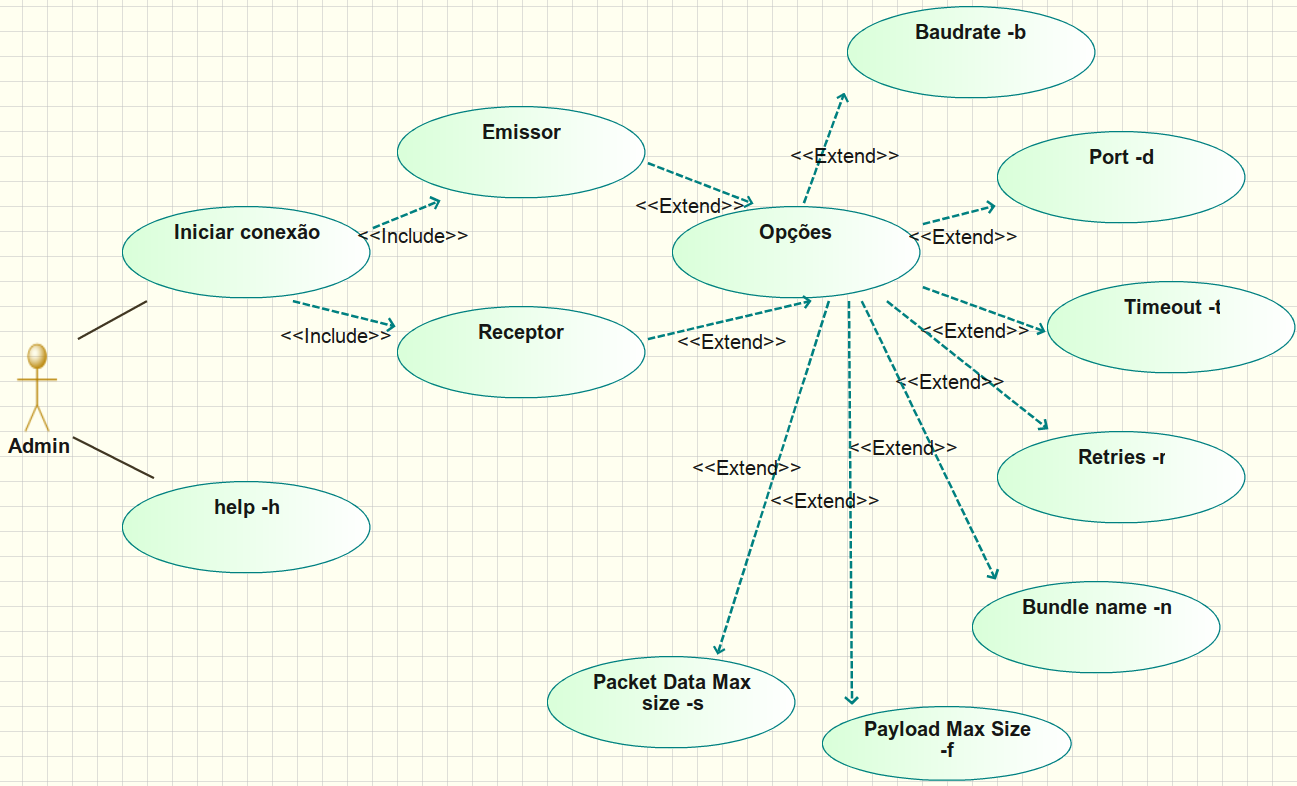
\includegraphics[scale=0.45]{useCases.png}}

\section{Protocolo de ligação lógica}
%identificação dos principais aspectos funcionais; descrição da estratégia de
%implementação destes aspectos com apresentação de extratos de código
Optámos por construir uma função, \textit{readCMD}, que implementa uma máquina de estados onde são
identificadas tramas válidas e em que o tipo controlo(C) é retornado por
argumento, que só deve ser usado guando o retorno desta função é verdadeiro
(indica que recebeu alguma trama bem formada). Assim, evitámos estar a
construir diversas máquinas de estados parecidas para as funções do linklayer.
O que iria dificultar a compreensão do código, a sua manutenibilidade e a
possível expansão do protocolo.\\\newline
Também foi tido em atenção o performance da aplicação, por exemplo: na função
\textit{readCMD} vamos fazendo o destuffing e calculando o BCC à medida que recebemos
nova informação, isto permite reduzir o número de ciclos. Usamos esta técnica
em todos os casos.

\begin{verbatim}
static bool readCMD(uint8_t * C) {

    ...

    while (!alarmed) {
        res = read(linkLayer.serialFileDescriptor, &ch, 1);

        if(res == 0)
            state = START;
        else if ( res == 1 ) {
            fprintf(stderr, "State: %d      Res: %lu      C: %X\n", state, res, ch);
            switch (state) {
            case START:
                if (ch == F)
                    state = F_RCV;
                break;
            case F_RCV:
                if (ch == A_CSENDER_RRECEIVER) {
                    state = A_RCV;
                    BCC1 = ch;
                } else if (ch != F)
                    state = START;
                break;
            case A_RCV:
                if (ch == F)
                    state = F_RCV;
                else {
                    if (isCMD(ch) || isCMDI(ch)) {
                        BCC1 ^= ch;
                        *C = ch;
                        state = C_RCV;
                    } else
                        state = START;
                }
                break;
            case C_RCV:
                 //headerErrorTest = random_bool(0.15); // Gerador de erros 15% probabilidade
                 if( headerErrorTest ) {   //Random error generator
                        fprintf(stderr, "Erro aleatório, header tem erros\n");
                        BCC1 ^= 0x05;
                        headerErrorTest = false;
                 }

                if (stuffing) { //Destuffing in run-time
                    stuffing = false;
                    if ((ch ^ STUFFING_XOR_BYTE) == BCC1) {
                        state = BCC_OK;
                    }
                    else
                         state = START;

                } else if (ch == ESC) {
                    stuffing = true;
                } else if (ch == BCC1) {
                    state = BCC_OK;
                } else if (ch == F)
                    state = F_RCV;
                else
                    state = START;
                break;
            case BCC_OK:
                if (ch == F && isCMD(*C)) {
                    fprintf(stderr, "Received CMD: ");
                    print_cmd(*C);
                    fprintf(stderr, "\n");
                    return true;
                } else if (isCMDI(*C) && (ch != F) && linkLayer.is_receiver) {
                    linkLayer.frame[linkLayer.frameLength++] = F;
                    linkLayer.frame[linkLayer.frameLength++] = A_CSENDER_RRECEIVER;
                    linkLayer.frame[linkLayer.frameLength++] = *C;
                    linkLayer.frame[linkLayer.frameLength++] = BCC1;
                    if ( ch == ESC ) {
                        stuffing = true;
                        BCC2 = 0x00;
                    } else {
                        linkLayer.frame[linkLayer.frameLength++] = ch;
                        BCC2 = ch;
                    }
                    state = RCV_I;
                    fprintf(stderr, "Receiving Frame I\n");
                } else
                    state = START;
                break;
            case RCV_I:
                if (linkLayer.frameLength >= (linkLayer.settings->payloadSize + 6)) {
                    fprintf(stderr, "This payload is invalid cause\
                    it exceeds the max number of bytes\n");
                    linkLayer.frameLength = 0;
                    if (ch == F)
                        state = F_RCV;
                    else
                        state = START;
                } else if ( (ch == F) && stuffing ) {
                    state = F_RCV;
                    linkLayer.frameLength = 0;
                    stuffing = false;
                } else if (ch == F) {
                    //Gerador de erros em software no campo de dados
                    //bodyErrorTest = random_bool(0.30);
                    if( bodyErrorTest ) {
                        fprintf(stderr, "Erro aleatório, body tem erros\n");
                        BCC2 ^= 0x05;
                        bodyErrorTest = false;
                    }
                    // Reverter, pois o ultimo é o BCC
                    BCC2 ^= linkLayer.frame[linkLayer.frameLength - 1];
                    if (BCC2 == linkLayer.frame[linkLayer.frameLength - 1]) {
                        linkLayer.frame[linkLayer.frameLength++] = ch;
                        fprintf(stderr, "Received Frame I, Length: %lu\n",\
                        linkLayer.frameLength);
                    }
                    return true;
                    // Uma vez que tem o cabeçalho da header válido, Rej e RR,
                    // fora ele verifica se o último elemento é F ou não
                } else if (stuffing) {  //Destuffing in run-time
                    stuffing = false;
                    temp = ch ^ STUFFING_XOR_BYTE;
                    linkLayer.frame[linkLayer.frameLength++] = temp;
                    BCC2 ^= temp;
                } else if (ch == ESC) {
                    stuffing = true;
                } else {
                    BCC2 ^= ch;
                    linkLayer.frame[linkLayer.frameLength++] = ch;
                }
                break;
            default:
                return false;
                break;
            }
        }
    }
    return false;
}
\end{verbatim}

Como podemos constatar esta função fica um pouco complexa.Ao invés das outras
funções do linkLayer.\\

\begin{verbatim}
int llwrite(uint8_t *packet, size_t packetSize) {

    ...

    while (tries < linkLayer.settings->numAttempts) {
        alarmed = false;
        received = false;

        fprintf(stderr, "Sending frame, Tries: %d\n", tries);
        res = write(linkLayer.serialFileDescriptor, stuffedFrame,
                stuffedFrameSize);
        if (res < 1) {
                    tries++;
                    continue;
        }
        alarm(linkLayer.settings->timeout);

        received = readCMD(&C);

        fprintf(stderr, "Receive: %d\n", received);
        if (received) {
            tries = 0;
            if ( C == (C_RR_RAW | (linkLayer.sequenceNumber << 7)) ) { // RR Errado
            } else if ( C == (C_RR_RAW | (changeSequenceNumber() << 7)) ) { // RR Certo
                linkLayer.sequenceNumber = changeSequenceNumber();
                free(stuffedFrame);
                linkLayer.reg.numFramesI++;
                return 0;
            } else if ( C == (C_REJ_RAW | (linkLayer.sequenceNumber << 7)) ) { //REJ Certo
                linkLayer.reg.numREJ++;
            } else if ( C == (C_REJ_RAW | (linkLayer.sequenceNumber << 7)) ) {//REJ Errado
            } else if ( C == C_DISC) {
                fprintf(stderr, "llwrite(): Receiver failed, trying again\n");
                break;
            } else {
                fprintf(stderr, "Received an unexpected command\n");
            }
        }
        tries++;
        linkLayer.reg.numFramesIResent++;
    }

    free(stuffedFrame);
    return -1;
}
\end{verbatim}

\begin{verbatim}
uint8_t* llread(size_t *payloadSize) {

    ...

    while (tries < linkLayer.settings->numAttempts) {
        fprintf(stderr, "Receiving frame\n");
        alarmed = false;
        alarm(linkLayer.settings->timeout);
        received = readCMD(&C);
        errno = 0;

        if (tries == 0) previousC = C;

        if (received) {
            if (!blockedSet) {
                if ( C == C_SET ) // Transmitter não recebeu bem o UA
                    res = write(linkLayer.serialFileDescriptor, uaCmd, uaCmdSize);
                else if ( !isCMDI(C) )// Se não for uma trama de informação
                    // O ruído pode 'construir' uma trama sem erros não esperada!
                    fprintf(stderr, "Garbage command received");
                else blockedSet = true;
            }
            if (blockedSet) {
                if ( (C == (C_I_RAW | (linkLayer.sequenceNumber << 6))) && \
                (linkLayer.frame[linkLayer.frameLength-1] != F) ) { //REJ
                    fprintf(stderr, "Cabeça da trama I boa, resto mau, mesma sequência -> rej\n");
                    linkLayer.reg.numREJ++;
                    if (linkLayer.sequenceNumber)
                        res = write(linkLayer.serialFileDescriptor, rej1Cmd, rej1CmdSize);
                    else
                        res = write(linkLayer.serialFileDescriptor, rej0Cmd, rej0CmdSize);
                    if (res < 1) {
                        tries++;
                        continue;
                    }
                    linkLayer.reg.numFramesIResent++;
                } else if ( (C == (C_I_RAW | (changeSequenceNumber() << 6))) &&
                \(linkLayer.frame[linkLayer.frameLength-1] != F) ) { //RR
                    fprintf(stderr, "Cabeça da trama I boa, resto mau, \
                    sequência diferente -> rr\n");
                    if (linkLayer.sequenceNumber)
                        res = write(linkLayer.serialFileDescriptor, rr1Cmd, rr1CmdSize);
                    else
                        res = write(linkLayer.serialFileDescriptor, rr0Cmd, rr0CmdSize);
                    if (res < 1) {
                        tries++;
                        continue;
                    }
                // Trama I esperada
                } else if ( C == (C_I_RAW | (linkLayer.sequenceNumber << 6)) ) {
                    fprintf(stderr, "Trama I esperada\n");
                    tempSize = linkLayer.frameLength - 6;
                    payloadToReturn = (uint8_t *) malloc( sizeof(uint8_t) * tempSize );
                    if ( payloadToReturn == NULL ) {
                        fprintf(stderr, "errno Enomem\n");
                        errno = ENOMEM;
                        goto cleanUp;
                    }
                    for (i = 0; i < tempSize; ++i) {
                        payloadToReturn[i] = linkLayer.frame[i+4];
                    }
                    *payloadSize = tempSize;
                    linkLayer.sequenceNumber = changeSequenceNumber();
                    if ( linkLayer.sequenceNumber == 0 )
                        res = write(linkLayer.serialFileDescriptor, rr0Cmd, rr0CmdSize);
                    else
                        res = write(linkLayer.serialFileDescriptor, rr1Cmd, rr1CmdSize);
                    if (res < 1) {
                        tries++;
                        continue;
                    }
                    linkLayer.reg.numFramesI++;
                    return payloadToReturn;
                    // Trama I duplicada, emissor nao recebeu a confirmação
                    //a tempo ou a confirmação foi perdida na rede
                } else if ( C == (C_I_RAW | (changeSequenceNumber() << 6)) ) {
                    if ( linkLayer.sequenceNumber == 0 )
                        res = write(linkLayer.serialFileDescriptor, rr0Cmd, rr0CmdSize);
                    else
                        res = write(linkLayer.serialFileDescriptor, rr1Cmd, rr1CmdSize);
                    if (res < 1) {
                        tries++;
                        continue;
                    }
                    fprintf(stderr, "Trama duplicada");
                } else if ( C == C_DISC ) { // Transmitter já enviou tudo
                    fprintf(stderr, "LLread received valid disconnect\n");
                    goto cleanUp;
                } else { // Recebeu uma trama de supervisão ou não numerada
                        // válida mas não esperada, ruído tramado!
                    if ( linkLayer.sequenceNumber == 0 )
                        res = write(linkLayer.serialFileDescriptor, rr0Cmd, rr0CmdSize);
                    else
                        res = write(linkLayer.serialFileDescriptor, rr1Cmd, rr1CmdSize);
                    if (res < 1) {
                        tries++;
                        continue;
                    }
                    fprintf(stderr, "Não esperava esta trama");
                }
            }
        }
        if (previousC == C || !received) ++tries;
        else tries = 0;
        previousC = C;
    }

    fprintf(stderr, "errno Econnaborted\n");
    errno = ECONNABORTED;

    cleanUp:
    ...
    return NULL;
}
\end{verbatim}

\begin{verbatim}
int llopen(void) {

    ...

    while (tries < linkLayer.settings->numAttempts) {
        alarmed = false;
        if (linkLayer.is_receiver) {
            alarm(linkLayer.settings->timeout);
            received = readCMD(&C);
            if (received && C == C_SET) {
                res = write(linkLayer.serialFileDescriptor, cmd, cmdSize);
                if (res < 1) {
                    tries++;
                    continue;
                }
                free(cmd);
                return 0;
            }
        } else {
            res = write(linkLayer.serialFileDescriptor, cmd, cmdSize);
            if (res < 1) {
                    tries++;
                    continue;
            }
            alarm(linkLayer.settings->timeout);
            received = readCMD(&C);
            if (received && C == C_UA) {
                free(cmd);
                return 0;
            }
        }

        tries++;
    }

    ...

    return -1;
}
\end{verbatim}

\begin{verbatim}
int llclose(void) {

    ...

    if ( !success ) {
        while (tries < linkLayer.settings->numAttempts) {
            alarmed = false;
            if (linkLayer.is_receiver) {
                res = write(linkLayer.serialFileDescriptor, DISC, DISCsize);
                if (res < 1) {
                    tries++;
                    continue;
                }
                alarm(linkLayer.settings->timeout);
                received = readCMD(&C);
                if (received && C == C_UA) {
                    fprintf(stderr, "Receiver in llclose received C_UA\n");
                    success = true;
                    goto cleanSerial;
                }
            } else {
                res = write(linkLayer.serialFileDescriptor, DISC, DISCsize);
                if (res < 1) {
                        tries++;
                        continue;
                }
                alarm(linkLayer.settings->timeout);
                received = readCMD(&C);
                if (received && C == C_DISC) {
                    res = write(linkLayer.serialFileDescriptor, UA, UAsize);
                    if (res < 1) {
                        tries++;
                        continue;
                    }
                    success = true;
                    goto cleanSerial;
                }
            }
            tries++;
        }
    }

    cleanSerial:

    ...

}
\end{verbatim}

Todas as funções que não estão aqui, tirando a \textit{llinitialize}, têm o
propósito de auxiliar a API do linkLayer. Foram removidas as declarações das
variáveis, criação das tramas, limpeza da memória alocada, tratamento de erros,
etc, de modo a não sobrecarregar o relatório.
%Falar sobre a máquina de estados; poupança de ciclos for, destuffing e bbc;
%mostrar o código da máquina de estados, llwrite, llread. Ligação entre funções
%do linklayer

\section{Protocolo de aplicação}
%identificação dos principais aspectos funcionais; descrição da estratégia de
%implementação destes aspectos com apresentação de extractos de código
A appLayer só necessita de ter uma função public visto que só tem de receber os
settings do parser. A partir daí a appLayer agarra a execução até haver uma
saturação do número de tentativas para a transferência do ficheiro(recuperação
em caso de erros), ou caso acha sucesso na transmissão/recepção.

\begin{verbatim}
int initAppLayer(Bundle *bundle) {

    ...

    for (tries = 0; tries < bundle->llSettings.numAttempts; ++tries) {
        llinitialize(&(bundle->llSettings), IS_RECEIVER(appLayer.settings->status));

        if(tries > 0)
            fprintf(stderr, "Recuperação de erro: %d\n", tries);

        if ( llopen() != 0 ) {
            fprintf(stderr, "Error: llopen()\n");
            llclose();
            continue;
        }
        else fprintf(stderr, "llopen() was successful\n\n");

        appLayer.sequenceNumber = 0;

        if ( IS_RECEIVER(appLayer.settings->status) ) {
            res = read();
            if ( res != 0 ) {
                fprintf(stderr, "There was an error in applayer read function\n");
                llclose();
                continue;
            }
        } else {
            res = write();
            if ( res != 0 ) {
                fprintf(stderr, "There was an error in applayer write function\n");
                llclose();
                continue;
            }
        }

        if( llclose() != 0) {
            fprintf(stderr, "Error: llclose(), going to exit\n");
                return -1;
        }
        else fprintf(stderr, "llclose() was successful\n");

        break;
    }

    if ( appLayer.settings->status == STATUS_TRANSMITTER_FILE || \
         appLayer.settings->status == STATUS_RECEIVER_FILE )
        fclose(appLayer.settings->io.fptr);

    if (tries < bundle->llSettings.numAttempts) {
         fprintf(stderr, "\n\nO ficheiro foi transferido com sucesso!\
         \nNúmero de tentativas: %d\n", tries);
    }
    else {
         fprintf(stderr, "\n\nO ficheiro não conseguiu transferido!\n");
    }

    return 0;
}
\end{verbatim}

\begin{verbatim}
static int read(void) {
    uint8_t *packet;
    size_t packetSize;
    size_t i;

    while (1) {
        packet = llread(&packetSize);
        if ( errno != 0 ) {
            fprintf(stderr, "AppRead received llread with error\n");
            return -1;
        } else {
            if ( packet == NULL ) {
                fprintf(stderr, "AppRead received disconnect from llread\n");
                return 0;
            } else {
                fprintf(stderr, "AppRead packet: ");
                for (i = 0; i < packetSize; i++) {
                    fprintf(stderr, "%X", packet[i]);
                }
                fprintf(stderr, "\n");
                if ( parserPacket(packet, packetSize) != 0 ) {
                    fprintf(stderr, "AppRead parserPacket failed\n");
                    return -1;
                }
            }
        }
    }
    return 0;
}
\end{verbatim}

\begin{verbatim}
static int write(void) {
    size_t res;
    bool end = false;
    uint8_t data[appLayer.settings->packetBodySize];
    size_t stringSize, lidos = 0;
    size_t databytesWritten = 0;

    if ( appLayer.settings->status == STATUS_TRANSMITTER_STRING )
        stringSize = strlen(appLayer.settings->io.chptr) + 1;
    else if ( appLayer.settings->status == STATUS_TRANSMITTER_FILE ) {
        if ( writeStartPacket() != 0 ) {
            fprintf(stderr, "writeStartPacket Failed\n");
            return -1;
        }
        rewind(appLayer.settings->io.fptr);
    }

    while ( !end ) {
        if ( appLayer.settings->status == STATUS_TRANSMITTER_FILE ) {
            res = fread(data, 1, appLayer.settings->packetBodySize, appLayer.settings->io.fptr);
            if ( feof(appLayer.settings->io.fptr) ) {
                fprintf(stderr, "AppWrite Reached end of file\n");
                end = true;
            } else if ( ferror(appLayer.settings->io.fptr) ) {
                fprintf(stderr, "AppWrite error occurred in fread\n");
                return -1;
            } else {
                fprintf(stderr, "AppWrite Res: %lu\n", res);
                fprintf(stderr, "AppWrite packet data: ");
                fprintf(stderr, "%.*s\n", (int)res, data);
            }
        } else if ( appLayer.settings->status == STATUS_TRANSMITTER_STRING ) {
            if ( (res = stringSize - lidos) <= appLayer.settings->packetBodySize ) {
                memcpy(data, appLayer.settings->io.chptr+lidos, res);
                fprintf(stderr, "AppWrite Reached end of string\n");
                end = true;
            } else {
                memcpy(data, appLayer.settings->io.chptr+lidos, \
                appLayer.settings->packetBodySize);
                lidos += appLayer.settings->packetBodySize;
                res = appLayer.settings->packetBodySize;
            }
            fprintf(stderr, "AppWrite packet: %s\n", data);
        } else {
            // Por fazer, ler stream
            // Não vai chegar aqui porque retorna -1 no llinitialize
            // Fiz dessa maneira pq talvez não vai dar tempo para implementar
        }
        if ( res != 0 ) {
            if ( writeDataPacket(data, res) == -1 ) {
                fprintf(stderr, "AppWrite Number of data bytes written so far: \
                %lu\n", databytesWritten);
                fprintf(stderr, "AppWrite failed\n");
                return -1;
            }
            databytesWritten += res;
        }
    }

    // Envia o tamanho do ficheiro ou da string
    if ( writeEndPacket() != 0 ) {
        fprintf(stderr, "writeEndPacket failed");
        return -1;
    }

    fprintf(stderr, "\n\nAppWrite Number of bytes Written: %lu\n\n", databytesWritten);
    return 0;
}
\end{verbatim}

\section{Validação}
%descrição dos testes efectuados com apresentação quantificada dos resultados,
%se possível
A técnica de teste dos programas foi feita à medida em que o código ia sendo
escrito. Na maior parte das vezes através de printfs. No entanto, também usámos
o gdb para testar o parser e algumas outras partes do código. Ademais, muitas
vezes tentámos isolar funções para tentar testá-las até à exaustão, por exemplo
mandando umas quantas strings e depois fazendo diffs. De início configurámos duas
máquinas virtuais para correr os testes, no entanto, isso provou ser bastante
chato. Por essa razão, encontrámos um software chamado socat que cria portas
série virtuais. sudo socat PTY,link=/dev/tty100,echo=0
PTY,link=/dev/tty200,echo=0 \&. Foi só na semana da apresentação que testámos o
nosso software no metal, felizmente funcionou tudo como ansiávamos.

%falar sobre os printfs; tentativa de fazer debugging com break points;
%vericacao da implementacao atraves de portas serie virtuais, socat; e nos pcs
%da feup

\section{Elementos de valorização}
%identificação dos elementos de valorização implementados; descrição da
%estratégia de implementação com apresentação de pequenos extratos de código
A seleção de parâmetros pelo utilizador por feita muito para além das exigências
pedidas.
\begin{verbatim}
Bundle** parse_args(int argc, char **argv, size_t *NBundles) {

    ...

    for (i = 0; i < *NBundles; ++i) {
        ioSet = false;
        if (*NBundles != 1) {
            subArgc = 0;
            oldSubArgv = subArgv;
            while ((subArgv < (argv + argc))
                    && ((strncmp(*subArgv, "+", 1) != 0) || subArgc == 0)) {
                ++subArgv;
                ++subArgc;
            }
        }

        if ((i == 0) && (subArgc == argc) && (*NBundles != 1)) {
            errno = EINVAL;
            return NULL;
        }

        while ((c = getopt((int) subArgc, oldSubArgv, "N:b:d:t:r:n:S:R:m:f:s:xhD"))
                != -1) {

            if (c == 'b' || c == 't' || c == 'r' || c == 'f' || c == 's') {
                parsedNumber = parse_ulong(optarg, 10);
                if (parsedNumber == ULONG_MAX) {
                    fprintf(stderr, "-%c must be followed by a number\n", c);
                    return NULL;
                }
            } else if (c == 'S' || c == 'R' || c == 'x' || c == 'm' || c == 'D') {
                if (ioSet) {
                    fprintf(stderr, "There can only be a mode for each bunnel");
                    return NULL;
                }
                ioSet = true;
            }

            switch (c) {
            case 'N':
                if (checkNDuplication > 1) {
                    fprintf(stderr, "There can only be a -N option");
                    errno = EINVAL;
                    return NULL;
                }
                ++checkNDuplication;
                break;
            case 'b':
                Bundles[i]->llSettings.baudRate = (tcflag_t) parsedNumber;
                break;
            case 'd':
                /* Regex testing */
                /*retn = regexec(&deviceRegex, optarg, 0, NULL, 0);*/
                /*if ( retn == REG_NOMATCH || retn != 0 ) {*/
                /*fprintf(stderr, "Not a proper device file, expected /dev/ttyS[0-9]+");*/
                /*errno = EINVAL;*/
                /*return NULL;*/
                /*}*/
                Bundles[i]->llSettings.port = optarg;
                break;
            case 't':
                Bundles[i]->llSettings.timeout = (unsigned int) parsedNumber;
                break;
            case 'r':
                Bundles[i]->llSettings.numAttempts =
                        (unsigned int) parsedNumber;
                break;
            case 'n':
                Bundles[i]->name = optarg;
                break;
            case 'S':
                if ((Bundles[i]->alSettings.io.fptr = fopen(optarg, "rb"))
                        == NULL) {
                    fprintf(stderr, "Error opening the file for reading\n");
                    return NULL;
                }
                Bundles[i]->alSettings.status = STATUS_TRANSMITTER_FILE;
                ptr = strrchr(optarg, '/');
                if (ptr == NULL)
                    Bundles[i]->alSettings.fileName = optarg;
                else
                    Bundles[i]->alSettings.fileName = ++ptr;
                break;
            case 'R':
                if ((Bundles[i]->alSettings.io.fptr = fopen(optarg, "w+b"))
                        == NULL) {
                    fprintf(stderr, "Error opening the file for writing\n");
                    return NULL;
                }
                Bundles[i]->alSettings.status = STATUS_RECEIVER_FILE;
                ptr = strrchr(optarg, '/');
                if (ptr == NULL)
                    Bundles[i]->alSettings.fileName = optarg;
                else
                    Bundles[i]->alSettings.fileName = ++ptr;
                break;
            case 'm':
                Bundles[i]->alSettings.io.chptr = optarg;
                Bundles[i]->alSettings.status = STATUS_TRANSMITTER_STRING;
                break;
            case 'f':
                Bundles[i]->llSettings.payloadSize =
                        (unsigned int) parsedNumber;
                break;
            case 's':
                Bundles[i]->alSettings.packetBodySize =
                        (unsigned int) parsedNumber;
                break;
            case 'x':
                Bundles[i]->alSettings.status = STATUS_TRANSMITTER_STREAM;
                break;
            case 'D':
                Bundles[i]->alSettings.status = STATUS_RECEIVER_FILE_RECEIVED_NAME;
                break;
            default:
                errno = EINVAL;
                return NULL;
                break;
            }
        }
        optind = 1;
        if (!ioSet)
            Bundles[i]->alSettings.status = STATUS_RECEIVER_STREAM;
    }

    return Bundles;
}
\end{verbatim}

\section{Conclusões}
%síntese da informação apresentada nas secções anteriores; reflexão sobre os
%objectivos de aprendizagem alcançados

\end{document}
